\section{РЕАЛИЗАЦИЯ КОМПОНЕНТОВ ПЛАТФОРМЫ}

После проектирования архитектуры следующим этапом стала реализация компонентов платформы. В соответствии с выбранной декомпозицией кодовая база разделена на четыре сервиса: \texttt{ParserSvc}, \texttt{InventorySvc}, \texttt{DriftDetectorSvc} и \texttt{ReconcilerSvc}. Каждый сервис реализует отдельную часть control loop и взаимодействует с остальными через HTTP API.

Реализация следует принципу разделения ответственности. Сервис разбора архитектурных манифестов не обращается к управляемым хостам, inventory-сервис не принимает решений о drift, сервис обнаружения drift не выполняет Ansible playbook, а reconciler не занимается построением desired state. Благодаря этому каждый компонент можно тестировать, развивать и расширять независимо.

\subsection{Реализация ParserSvc: загрузка Structurizr JSON, построение desired state, API}

\texttt{ParserSvc} реализован на Go и отвечает за преобразование Architecture-as-Code-описания в host-centric desired state. Компонентная структура сервиса представлена на рисунке~\ref{fig:ch3-parser-components}.

\begin{figure}
  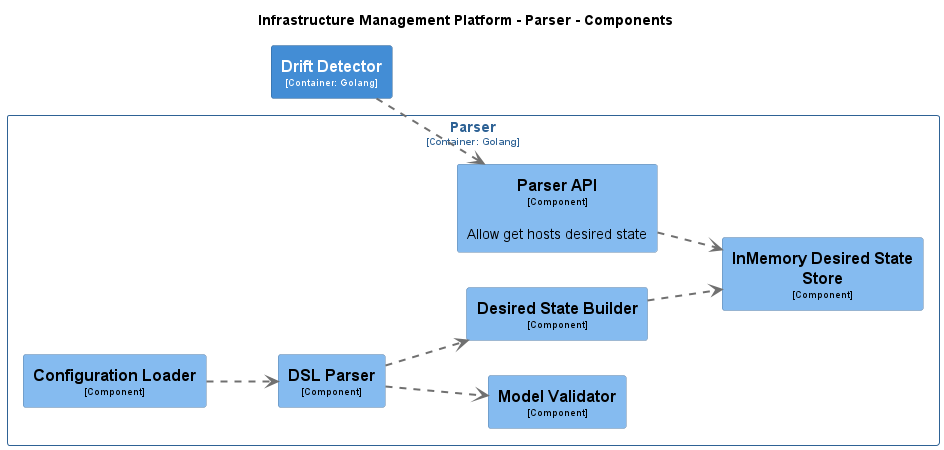
\includegraphics[width=0.95\linewidth]{../platform-arch-images/parser-components.png}
  \caption{Компонентная структура ParserSvc}
  \label{fig:ch3-parser-components}
\end{figure}

На уровне запуска сервис выполняет последовательность действий: загружает конфигурацию, определяет путь к манифестам, находит доступные JSON-файлы, разбирает каждый валидный файл, строит desired state и сохраняет его во внутреннем in-memory store. После этого поднимается HTTP API, через которое остальные компоненты платформы получают целевое состояние.

Конфигурация сервиса содержит параметры HTTP-сервера, уровень логирования и блок \texttt{manifests}. Для манифестов поддерживаются два режима: \texttt{file} и \texttt{directory}. В режиме \texttt{file} сервис обрабатывает один указанный файл. В режиме \texttt{directory} он просматривает верхний уровень директории и выбирает только файлы с расширением \texttt{.json}. Файлы с другими расширениями, включая \texttt{.dsl}, игнорируются. Такое решение связано с тем, что ParserSvc не является интерпретатором Structurizr DSL; он работает со структурированным JSON-представлением.

Разбор входного файла выполняется в два этапа. Сначала JSON десериализуется во внутреннюю структуру Structurizr-манифеста. Сервис проверяет наличие \texttt{model.deploymentNodes}, поскольку без deployment-узлов невозможно построить host-centric desired state. Затем mapper-слой преобразует элементы Structurizr-модели в доменную модель платформы.

Для сопоставления container instance с именем workload mapper строит карту контейнеров по \texttt{containerId}. Источником этой карты служит раздел \texttt{model.softwareSystems[].containers}. Далее сервис рекурсивно обходит deployment-узлы. Это важно, потому что Structurizr-модель может содержать вложенные deployment node, а инфраструктурно значимые хосты не всегда находятся только на верхнем уровне.

Для каждого deployment node извлекаются обязательные свойства: \texttt{host\_id}, \texttt{fqdn}, \texttt{env}, \texttt{managed\_by}, \texttt{purpose}. Поле \texttt{ip} является необязательным. Остальные свойства, не относящиеся к служебным полям Structurizr, преобразуются в labels. Таким образом, desired state сохраняет как минимально обязательные атрибуты, так и дополнительные признаки хоста: регион, владельца, роль или иные эксплуатационные метки.

Workload строится на основе container instance. Обязательными полями являются имя контейнера, \texttt{enabled} и \texttt{deployment\_mode}. Если режим развертывания равен \texttt{container}, обязательным становится поле \texttt{image}. Дополнительно поддерживаются \texttt{version} и \texttt{port}.

Итоговое состояние сохраняется в in-memory store как snapshot. Store возвращает копии данных, что защищает внутреннее состояние от случайного изменения вызывающим кодом. В metadata snapshot фиксируются время загрузки, режим и путь манифестов, количество найденных, загруженных, поврежденных и проигнорированных файлов, общее число хостов и workload, а также readiness-статус.

HTTP API ParserSvc включает:
\begin{enumerate}
    \item \texttt{GET /healthz} --- проверка liveness;
    \item \texttt{GET /readyz} --- проверка готовности desired state;
    \item \texttt{GET /api/v1/desired-state} --- получение полного desired state;
    \item \texttt{GET /api/v1/desired-state/hosts} --- получение списка хостов с фильтрами;
    \item \texttt{GET /api/v1/desired-state/hosts/:hostId} --- получение одного хоста по идентификатору.
\end{enumerate}

Список хостов поддерживает фильтрацию по \texttt{fqdn} и labels. Несколько фильтров применяются с AND-семантикой. Это полезно для последующего расширения платформы, поскольку позволяет выбирать хосты по окружению, команде, назначению или другим признакам без изменения внутренней модели desired state.

\subsection{Реализация InventorySvc: selfProvisioning, cAdvisor, snapshot, partial result}

\texttt{InventorySvc} реализован на Go и отвечает за формирование actual state управляемых хостов. Компонентная структура сервиса представлена на рисунке~\ref{fig:ch3-inventory-components}.

\begin{figure}
  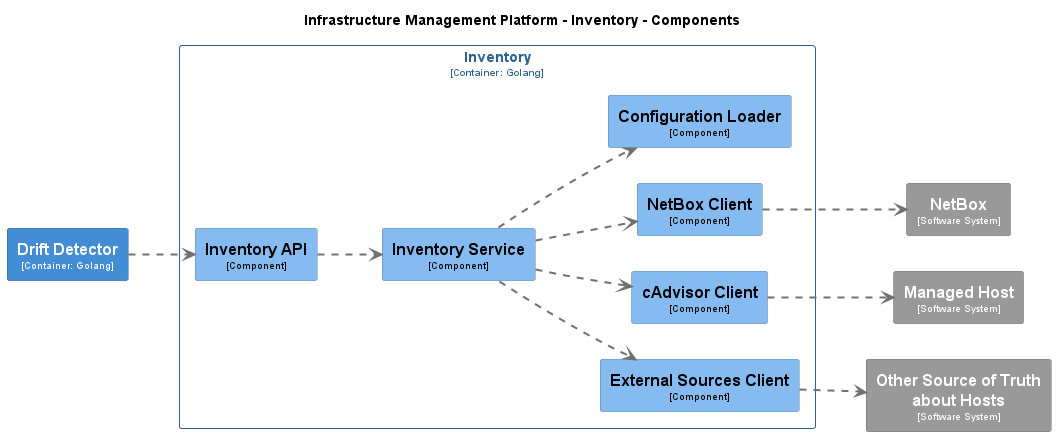
\includegraphics[width=0.95\linewidth]{../platform-arch-images/inventory-components.png}
  \caption{Компонентная структура InventorySvc}
  \label{fig:ch3-inventory-components}
\end{figure}

Сервис построен как canonical read-model фактического состояния. Он не обращается к cAdvisor при каждом HTTP-запросе. Вместо этого InventorySvc периодически выполняет синхронизацию, формирует snapshot и отдаёт через API уже подготовленные данные. Такой подход уменьшает зависимость потребителей API от мгновенной доступности внешних источников и делает ответы согласованными в пределах завершенного цикла синхронизации.

Начальная область наблюдения задается файлом \texttt{selfProvisioning}. Он содержит список хостов с полями \texttt{id}, \texttt{fqdn} и \texttt{labels}. Валидация требует уникальности \texttt{id} и \texttt{fqdn}, а также наличия обязательных labels: \texttt{managed\_by}, \texttt{purpose}, \texttt{env}. Таким образом, bootstrap-описание задает минимальную инвентарную основу, от которой сервис отталкивается при сборе actual state.

Фактические сведения о workload собираются через source-слой. Для каждого bootstrap-хоста сервис строит URL по шаблону из конфигурации и обращается к endpoint \texttt{/api/v1.3/subcontainers/}. Ответ cAdvisor нормализуется в доменную модель \texttt{Workload}. При этом из данных контейнера выделяются идентификатор, имя, image, runtime, источник и время последнего наблюдения.

Синхронизация InventorySvc выполняется как initial sync и periodic sync. Initial sync происходит до перехода сервиса в состояние ready. Periodic sync запускается по интервалу из конфигурации и обновляет snapshot. Внутреннее хранилище использует потокобезопасный доступ, поэтому API может читать предыдущее согласованное состояние, пока очередной цикл синхронизации готовит новое.

Особое внимание в реализации уделено partial result. Если источник данных недоступен для части хостов, InventorySvc не завершает работу ошибкой и не отбрасывает полностью результат синхронизации. Вместо этого он возвращает данные по доступным хостам, а для проблемных хостов фиксирует ошибки и статусы источников. На уровне metadata выставляются признаки \texttt{isPartial}, \texttt{failedHosts}, \texttt{lastSyncAt}, \texttt{lastFullSyncAt} и \texttt{lastPartialSyncAt}.

Статус хоста может принимать значения \texttt{ok}, \texttt{partial}, \texttt{error}, \texttt{bootstrap\_only}. Дополнительно для каждого источника хранится \texttt{sourceStatus}: включен ли источник, успешно ли он отработал, когда были получены данные и какая ошибка возникла при неуспехе. Именно эта информация затем используется DriftDetectorSvc для безопасного решения: можно ли считать actual state достаточно полным для обнаружения drift.

HTTP API InventorySvc включает:
\begin{enumerate}
    \item \texttt{GET /healthz} --- проверка liveness;
    \item \texttt{GET /readyz} --- проверка готовности после initial sync;
    \item \texttt{GET /api/v1/hosts} --- список хостов с metadata;
    \item \texttt{GET /api/v1/hosts/:id} --- карточка одного хоста.
\end{enumerate}

Список хостов поддерживает фильтрацию по labels с AND-семантикой. API возвращает не только workload, но и metadata snapshot, что позволяет потребителю учитывать полноту actual state. Для платформы это принципиально: качество решения о drift зависит не только от списка workload, но и от того, насколько достоверны данные источника.

\subsection{Реализация DriftDetectorSvc: клиенты, detector registry, cooldown, статистика цикла}

\texttt{DriftDetectorSvc} реализован на Go и является компонентом, который связывает desired state, actual state и reconcile. Его компонентная структура представлена на рисунке~\ref{fig:ch3-drift-detector-components}.

\begin{figure}
  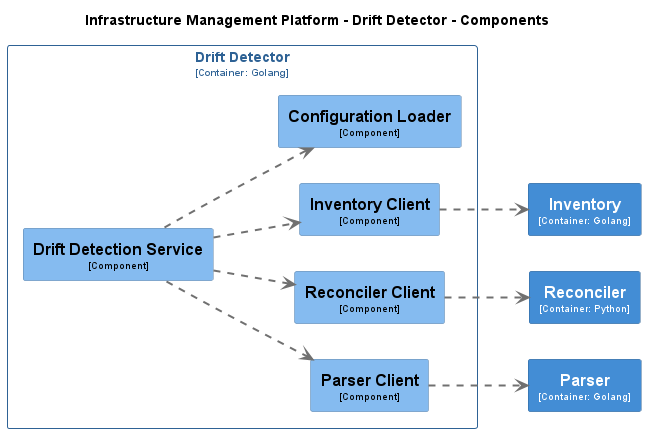
\includegraphics[width=0.95\linewidth]{../platform-arch-images/drift-detector-components.png}
  \caption{Компонентная структура DriftDetectorSvc}
  \label{fig:ch3-drift-detector-components}
\end{figure}

При запуске сервис загружает конфигурацию, инициализирует HTTP-клиенты для ParserSvc, InventorySvc и ReconcilerSvc, создает registry detector-ов и запускает первый detection cycle. После успешного цикла сервис считается ready. Дополнительно поддерживается периодический запуск по scheduler и ручной запуск одного цикла через API.

Detection cycle выполняется последовательно. Сначала сервис получает actual state, затем desired state. После этого он индексирует actual-хосты по \texttt{host\_id} и \texttt{fqdn}. Для каждого desired-хоста выполняется поиск соответствующего actual-хоста. Приоритет отдается \texttt{host\_id}; если он не найден, используется \texttt{fqdn}. Если хост не найден, цикл помечается как partial, а данный хост пропускается.

Далее для каждого включенного компонента вызывается соответствующий detector. Каждый detector реализует общий интерфейс и возвращает структурированный результат: применима ли проверка, отсутствуют ли actual-данные, найден ли drift, какое предупреждение сформировано и какую reconcile-команду следует отправить.

Detector \texttt{cadvisor} имеет особую bootstrap-семантику. Если desired state требует \texttt{cadvisor}, но источник cAdvisor для хоста недоступен, detector может сформировать reconcile-команду на установку cAdvisor. Такое поведение оправдано тем, что cAdvisor является не только управляемым workload, но и источником actual state для последующих проверок.

После обнаружения drift DriftDetectorSvc формирует reconcile-команду. В команду входят \texttt{host\_id}, \texttt{fqdn}, \texttt{component}, \texttt{correlation\_id} и параметры компонента. Для \texttt{node\_exporter} это могут быть \texttt{node\_exporter\_image} и \texttt{node\_exporter\_port}; для \texttt{cadvisor} --- \texttt{cadvisor\_image} и \texttt{cadvisor\_port}. \texttt{correlation\_id} строится из идентификатора detection cycle, компонента и FQDN, что упрощает трассировку действий в логах.

Перед отправкой команды применяется cooldown-хранилище. Оно реализовано как in-memory map вида \texttt{component|fqdn -> lastSentAt}. Если с момента последней отправки прошло меньше заданного интервала, команда подавляется. В статистике цикла увеличивается счетчик \texttt{reconcileSuppressed}. Если отправка разрешена и ReconcilerSvc вернул \texttt{202 Accepted}, команда считается принятой, а ключ cooldown обновляется.

Результат каждого цикла сохраняется как \texttt{DetectionCycleResult}. В нем фиксируются идентификатор цикла, trigger, время начала и завершения, длительность, stage timings, признаки partial, готовность ParserSvc, статистика и списки предупреждений/ошибок. Stage timings включают время получения inventory, время получения desired state, время сравнения drift и время отправки reconcile-команд.

HTTP API DriftDetectorSvc включает:
\begin{enumerate}
    \item \texttt{GET /healthz} --- liveness;
    \item \texttt{GET /readyz} --- readiness на основе успешного detection cycle;
    \item \texttt{POST /api/v1/detection/run} --- запуск одного detection cycle.
\end{enumerate}

Для ручного запуска реализована защита от параллельного выполнения. Если detection cycle уже идет, сервис возвращает \texttt{409 Conflict}. Это важно для согласованности статистики и для предотвращения одновременной отправки одинаковых reconcile-команд.

\subsection{Реализация ReconcilerSvc: FastAPI, очередь, operators, Ansible Runner}

\texttt{ReconcilerSvc} реализован на Python с использованием FastAPI. Сервис принимает reconcile-команды, валидирует их, выбирает operator, строит execution plan и ставит задачу во внутреннюю очередь. Компонентная структура сервиса представлена на рисунке~\ref{fig:ch3-reconciler-components}.

\begin{figure}
  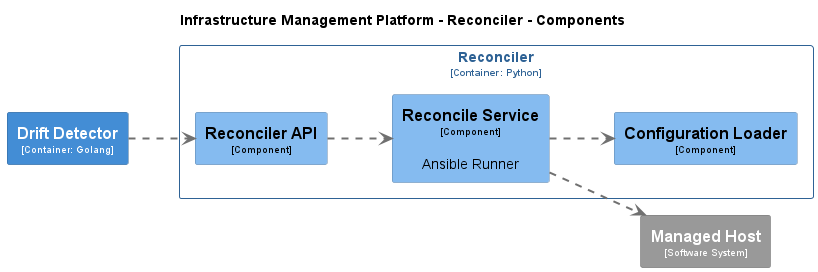
\includegraphics[width=0.95\linewidth]{../platform-arch-images/reconciler-components.png}
  \caption{Компонентная структура ReconcilerSvc}
  \label{fig:ch3-reconciler-components}
\end{figure}

HTTP API сервиса содержит \texttt{GET /healthz}, \texttt{GET /readyz} и \texttt{POST /api/v1/reconcile}. Основной запрос описан моделью \texttt{ReconcileRequest}. Обязательными полями являются \texttt{fqdn} и \texttt{component}. Дополнительно могут передаваться \texttt{host\_id}, \texttt{correlation\_id} и словарь \texttt{parameters}. Для FQDN выполняется валидация допустимых символов.

При успешном принятии запроса сервис возвращает \texttt{ReconcileAcceptedResponse} со статусом \texttt{accepted}, \texttt{request\_id}, компонентом, FQDN, \texttt{correlation\_id} и временем принятия. Важно, что ответ \texttt{202 Accepted} означает только постановку задачи в очередь. Он не означает, что workload уже установлен или что Ansible playbook завершился успешно.

Основная бизнес-логика сосредоточена в \texttt{ReconcileService}. Сервис генерирует \texttt{request\_id}, логирует входящий запрос, выбирает operator через \texttt{OperatorRegistry}, строит execution plan и передает задачу в очередь. Если очередь переполнена или не готова принимать задачи, API возвращает \texttt{503}. Если operator не найден, возвращается ошибка клиентского запроса. Если execution plan не может быть построен, возвращается серверная ошибка.

Operator-слой состоит из базового интерфейса \texttt{ReconcileOperator}, registry и конкретных operator-ов. Каждый operator знает, какой playbook использовать и какие default parameters применить. При построении execution plan default-параметры объединяются с параметрами, полученными от DriftDetectorSvc. Это позволяет detector-у передать image или port из desired state, не меняя общий контракт ReconcilerSvc.

Выполнение playbook изолировано в \texttt{AnsibleRunnerAdapter}. Adapter читает SSH-параметры из переменных окружения, строит in-memory inventory для целевого FQDN, добавляет служебные extra vars и запускает Ansible Runner \cite{ansible_docs}. Результат выполнения нормализуется до статуса, кода возврата, признака успешности и длительности. Потоковые события Ansible логируются со служебными полями \texttt{request\_id}, \texttt{component}, \texttt{fqdn} и \texttt{correlation\_id}.

Таким образом, ReconcilerSvc реализует управляемую асинхронную модель восстановления. Он отделяет прием команды от выполнения, ограничивает параллелизм, скрывает детали Ansible за adapter-слоем и предоставляет точку расширения через operator registry.

\subsection{Контракты API и взаимодействие сервисов}

Взаимодействие сервисов построено на явных HTTP-контрактах. Такой подход делает границы компонентов прозрачными и позволяет развивать внутреннюю реализацию сервисов без изменения их внешнего поведения.

Общий поток взаимодействия можно описать следующим образом. ParserSvc заранее формирует desired state из Structurizr JSON. InventorySvc формирует actual state на основе bootstrap-описания и данных источников наблюдения. DriftDetectorSvc обращается к обоим сервисам, нормализует полученные ответы в собственные доменные модели и применяет detector-ы. При подтвержденном drift DriftDetectorSvc отправляет reconcile-команду в ReconcilerSvc. ReconcilerSvc принимает команду, строит execution plan и асинхронно выполняет восстановление через Ansible Runner.

Проектная особенность состоит в том, что ни один сервис не обращается напрямую к внутреннему состоянию другого сервиса. ParserSvc и InventorySvc скрывают свои in-memory snapshot за API. DriftDetectorSvc не знает, как именно ParserSvc разбирает Structurizr JSON и как InventorySvc получает данные от cAdvisor. ReconcilerSvc не знает, по каким правилам был обнаружен drift; он работает с уже сформированной reconcile-командой.

Такая организация дает несколько инженерных преимуществ. Во-первых, упрощается тестирование: каждый сервис можно проверять через его публичные функции и HTTP-слой. Во-вторых, появляется возможность независимого расширения. Например, InventorySvc может получить новый источник данных, не меняя DriftDetectorSvc, если внешний контракт actual state сохранится. В-третьих, повышается надежность границ: ошибки получения actual state, ошибки разбора desired state и ошибки выполнения reconcile фиксируются в разных местах и не смешиваются в один монолитный процесс.

Итогом реализации стала связанная платформа, в которой каждый компонент выполняет собственную роль в общем цикле управления инфраструктурой. ParserSvc предоставляет целевое состояние из архитектурного описания, InventorySvc предоставляет наблюдаемое состояние, DriftDetectorSvc принимает решение о расхождении, а ReconcilerSvc выполняет восстановление поддержанных workload. В следующей главе рассматривается проверка качества разработанного решения и экспериментальная оценка ключевых характеристик платформы.
